% ==================///==================///==================///
% ==================/// LATEX'S STUFF
% ==================///==================///==================///

\documentclass[hungarian]{beamer}
\usepackage[T1]{fontenc}
\usepackage{babel}
\usepackage{graphicx}
\usepackage{hyperref}
\usepackage{stuki}

\usepackage{soul}

\usepackage{tikz}
\usetikzlibrary{shapes.multipart, positioning, arrows.meta}
\tikzset{list/.style={rectangle multipart, draw, minimum height=1cm, minimum width=1.5cm}}

\usepackage{amsfonts,amsmath,oldgerm}
\usetheme{_statale}
\usefonttheme[onlymath]{serif}

\newcommand{\testcolor}[1]{\colorbox{#1}{\textcolor{#1}{test}}~\texttt{#1}}
\newcommand{\hrefcol}[2]{\textcolor{cyan}{\href{#1}{#2}}}
\titlebackground*{assets/background}

\newcommand{\Ord}{\mathcal{O}}


% ==================///==================///==================///
% ==================/// SPLASH PAGE
% ==================///==================///==================///

\title{Algoritmusok I.}
\newcommand{\longauthor}{8. gyakorlat}
\author{Sipos Ágoston}
\newcommand{\correspondingauthor}{John Doe}
\newcommand{\email}{siposagoston@inf.elte.hu}
\renewcommand{\insertdate}{2026. november 4.}

% ==================///==================///==================///
% ==================/// START PRESENTATION
% ==================///==================///==================///

\newcommand{\bintree}{%
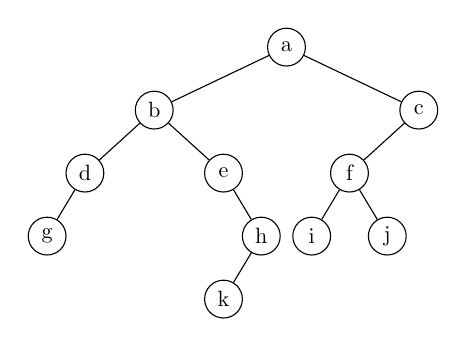
\begin{tikzpicture}[level distance=1cm, every node/.style={circle,draw,minimum size=6mm,inner sep=1pt},
 level 1/.style={sibling distance=4.2cm}, level 2/.style={sibling distance=2.2cm}, level 3/.style={sibling distance=1.2cm}, scale=0.8, transform shape]
\node {a}
 child { node {b}
   child { node {d} child { node {g} } child[missing] }
   child { node {e} child[missing] child { node {h} child { node {k} } child[missing] } } }
 child { node {c}
   child { node {f} child { node {i} } child { node {j} } }
   child[missing] };
\end{tikzpicture}}

\newcommand{\tasktree}{%
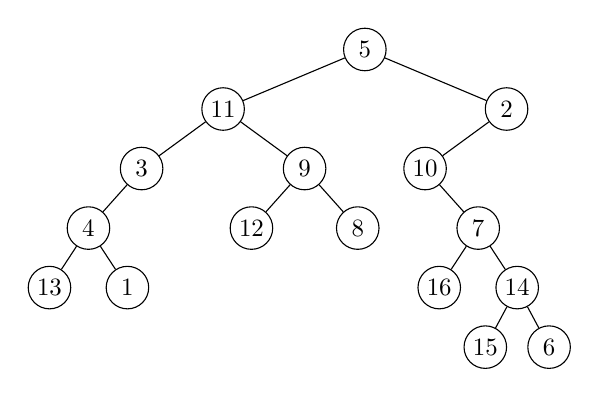
\begin{tikzpicture}[level distance=0.84cm, every node/.style={circle,draw,minimum size=6mm,inner sep=1pt},
 level 1/.style={sibling distance=4cm}, level 2/.style={sibling distance=2.3cm}, level 3/.style={sibling distance=1.5cm}, level 4/.style={sibling distance=1.1cm}, level 5/.style={sibling distance=0.9cm}, scale=0.9, transform shape]
\node {5}
 child { node {11}
   child { node {3}
     child { node {4} child { node {13} } child { node {1} } }
     child[missing] }
   child { node {9} child { node {12} } child { node {8} } } }
 child { node {2}
   child { node {10}
     child[missing]
     child { node {7}
       child { node {16} }
       child { node {14} child { node {15} } child { node {6} } } } }
   child[missing] };
\end{tikzpicture}}

\begin{document}
\maketitle

\section{Bináris fák}

\begin{frame}{Bináris fa ábrázolása}
\begin{columns}
\begin{column}{0.6\linewidth}
\begin{itemize}
    \item Láncolt ábrázolás
    \begin{itemize}
        \item két pointerrel: \texttt{left}, \texttt{right}
        \item három pointerrel: \texttt{left}, \texttt{right}, \texttt{parent}
    \end{itemize}
    \item Aritmetikai ábrázolás
    \begin{itemize}
        \item szintfolytonos elhelyezés egy tömbben
        \item bal-, jobb gyerek és szülő az indexekből számítható
        \item csak „tömör” fákra hatékony (lásd később: kupac)
    \end{itemize}
\end{itemize}
\end{column}
\begin{column}{0.4\linewidth}
\bintree
\end{column}
\end{columns}
\end{frame}

\begin{frame}{Láncolt ábrázolás}
\begin{columns}
\begin{column}{0.5\linewidth}
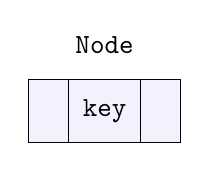
\begin{tikzpicture}[
    node/.style={rectangle split, rectangle split parts=3, rectangle split horizontal, draw, minimum height=0.8cm, inner sep=5pt, fill=blue!5}]
    \node[node] (a) {\nodepart{two} \texttt{key} \nodepart{three}};
    \node[above=0.2cm of a] {\texttt{Node}};
\end{tikzpicture}

\vspace{4mm}
\texttt{Node}: \texttt{left}, \texttt{key}, \texttt{right} (és esetleg \texttt{parent})
\end{column}
\begin{column}{0.5\linewidth}
\begin{tabular}{lll}
\hline
Ábrázolás & Művelet & Jelentés\\
\hline
$t \to left$ & $left(t)$ & bal részfa\\
$t \to right$ & $right(t)$ & jobb részfa\\
$t \to parent$ & $parent(t)$ & szülő\\
$t \to key$ & $key(t)$ & kulcs\\
$t = \emptyset$ & $t = \Omega$ & üres fa\\
\hline
\end{tabular}
\end{column}
\end{columns}
\end{frame}

\section{Bejárások}

\begin{frame}{Rekurzív bejárások}
\begin{columns}
\begin{column}{0.5\linewidth}
\bintree
\end{column}
\begin{column}{0.5\linewidth}
\begin{itemize}
    \item Preorder: gyökér, bal, jobb
    \item Inorder: bal, gyökér, jobb
    \item Postorder: bal, jobb, gyökér
    \item Szintfolytonos: szintenként, balról jobbra
\end{itemize}
\end{column}
\end{columns}
\end{frame}

\begin{frame}{Bejárási sorrendek}
\begin{columns}
\begin{column}{0.4\linewidth}
\bintree
\end{column}
\begin{column}{0.6\linewidth}
\small
Preorder: \texttt{a b d g e h k c f i j}

\vspace{2mm}
Inorder: \texttt{g d b e k h a i f j c}

\vspace{2mm}
Postorder: \texttt{g d k h e b i j f c a}

\vspace{2mm}
Szintfolytonos: \texttt{a b c d e f g h i j k}
\end{column}
\end{columns}
\end{frame}

\begin{frame}[t]{Feladat: bejárások 1.}
Add meg, milyen sorrendben írja ki az alábbi fa kulcsait a három rekurzív bejáró algoritmus!

\vspace{2mm}
\tasktree
\end{frame}

\begin{frame}[t]{Feladat: bejárások 2.}
Rekonstruáld a fát a következő post- és inorder bejárásból!

\vspace{3mm}
Postorder: \texttt{17, 4, 7, 9, 45, 91, 2, 8, 53, 10, 66, 72, 34, 5, 3}

Inorder: \texttt{17, 8, 4, 7, 91, 45, 9, 2, 3, 5, 34, 53, 66, 10, 72}
\end{frame}

\begin{frame}{Rekonstrukció}
\begin{itemize}
    \item Mi a fa gyökere? A postorder bejárás utolsó eleme.
    \item Mit tudunk az inorder bejárásból? A gyökértől balra álló elemek a bal, a jobbra állók a jobb részfában vannak.
    \item Ezt a részfákra is megismételjük.
\end{itemize}

\vspace{4mm}
Bármely két bejárásból rekonstruálható a fa?

\pause
\textbf{Nem}: a preorder--postorder pár nem elég. Egy gyerekes csúcsnál nem derül ki, hogy a gyerek bal vagy jobb gyerek.
\end{frame}

\section{Rekurzív algoritmusok}

\begin{frame}{Bináris fa magassága}
Egy leghosszabb ág éleinek száma. Üres fa magassága $-1$, egy csúcsé $0$.

\vspace{2mm}
Ötlet: $h(t) = \max(h(left(t)), h(right(t))) + 1$, $h(\Omega) = -1$

\vspace{2mm}
\setlength{\stukiwidth}{10cm}
\begin{stukibox*}{h(t : Node*) : $\mathbb{Z}$}
\begin{IF}[25]{1}{\stm{t = \emptyset}}
    \stm{return\; -1}
\ELSE
    \stm{return\; \max(h(t \to left), h(t \to right)) + 1}
\end{IF}
\end{stukibox*}
\end{frame}

\begin{frame}[t]{Feladat: magasság}
Határozzuk meg az alábbi fa magasságát, illetve tekintsük át, milyen lépéseket tesz az algoritmus!

\vspace{2mm}
\tasktree
\end{frame}

\begin{frame}{Levelek száma}
Ha $t$ levél, akkor $1$; különben a bal és jobb részfa leveleinek összege.

\vspace{2mm}
\setlength{\stukiwidth}{12cm}
\begin{stukibox*}{leaves(t : Node*) : $\mathbb{N}$}
\begin{IF}[25]{3}{\stm{t = \emptyset}}
    \stm{return\;0}
\ELSE
\begin{IF}[40]{2}{\stm{t \to left = \emptyset \textrm{ and } t \to right = \emptyset}}
    \stm{return\;1}
\ELSE
    \stm{return\;leaves(t \to left) +\\ leaves(t \to right)}
\end{IF}
\end{IF}
\end{stukibox*}
\end{frame}

\begin{frame}{Maximális kulcs 1. -- globális változóval}
Preorder bejárás közben egy \texttt{max} változót viszünk magunkkal (referencia szerint). Az üres fát külön kezeljük (hiba).

\vspace{2mm}
\setlength{\stukiwidth}{9cm}
\begin{stukibox*}{preorderMax(t : Node*; $\&$max : $\mathbb{Z}$)}
\begin{IF}[70]{4}{\stm{t \neq \emptyset}}
    \begin{IF}[50]{1}{\stm{t \to key > max}}
        \stm{max = t \to key}
    \ELSE
        \stm*{SKIP}
    \end{IF}
    \stm{preorderMax(t \to left, max)}
    \stm{preorderMax(t \to right, max)}
\ELSE
    \stm*{SKIP}
\end{IF}
\end{stukibox*}

\vspace{2mm}
Hívás: \texttt{max = t->key; preorderMax(t, max)}
\end{frame}

\begin{frame}[t]{Maximális kulcs 2. -- részfák eredményeiből}
Feladat: írjuk meg úgy, hogy a maximumot visszatérési értékként kapjuk! Előfeltétel: $t \neq \emptyset$. Figyeljünk a hiányzó gyerekekre!
\end{frame}

\begin{frame}[t]{Negatív kulcs keresése rekurzívan}
Feladat: függvény, mely egy negatív kulcsú csúcs címével tér vissza, ha nincs ilyen, akkor $\emptyset$-val.
\end{frame}

\section{Szintfolytonos bejárás}

\begin{frame}[t]{Szintfolytonos bejárás}
Sor segítségével.

\setlength{\stukiwidth}{9cm}
\begin{stukibox*}{levelOrder(t : Node*)}
\begin{IF}[85]{7}{\stm{t \neq \emptyset}}
    \stm{Q : Queue; Q.add(t)}
    \begin{WHILE}{5}{\stm{\neg Q.isEmpty()}}
        \stm{p = Q.rem(); process(p)}
        \begin{IF}[50]{1}{\stm{p \to left \neq \emptyset}}
            \stm{Q.add(p \to left)}
        \ELSE
            \stm*{SKIP}
        \end{IF}
        \begin{IF}[50]{1}{\stm{p \to right \neq \emptyset}}
            \stm{Q.add(p \to right)}
        \ELSE
            \stm*{SKIP}
        \end{IF}
    \end{WHILE}
\ELSE
    \stm*{SKIP}
\end{IF}
\end{stukibox*}
\end{frame}

\begin{frame}[t]{Szemléltetés}
Játsszuk le a szintfolytonos bejárást a fán! Mi lesz a sor tartalma lépésenként?

\bintree
\end{frame}

\begin{frame}[t]{Feladat: egygyerekes csúcsok}
Hány egygyerekes csúcsa van a fának a $0..k$ szinteken? Hány van a $k$-nál nagyobb szinteken?
\end{frame}

\iffalse
\begin{frame}[t]{Feladat: negatív kulcs szintfolytonosan}
Keressünk negatív kulcsú elemet szintfolytonos bejárással. Siker esetén az elemre mutató pointert, különben \texttt{NULL}-t adjunk vissza.
\end{frame}

\begin{frame}[t]{Feladat: levelek száma szintfolytonosan}
Számoljuk meg a fa leveleit szintfolytonos bejárással. (Trükk: ha $t$ levél, nincsenek leszármazottai, nem kell őket sorba tenni.)
\end{frame}
\fi

\begin{frame}{Szintszám nyilvántartása}
Feladat: írjuk ki a levelek kulcsát a szintszámmal együtt.

\vspace{2mm}
\textbf{Rossz megoldás:} egy számlálót növelünk minden kivett csúcsnál: ez a szintfolytonos \emph{sorszámot} adja, nem a szintet.

\vspace{2mm}
Megoldások:
\begin{itemize}
    \item $\langle Node*, \mathbb{N}\rangle$ párokat teszünk a sorba
    \begin{tabular}{|c|c|}
        \hline
        (b, 1) & (c, 1) \\
        \hline
    \end{tabular} $\rightarrow$
    \begin{tabular}{|c|c|c|}
        \hline
        (c, 1) & (d, 2) & (e, 2) \\
        \hline
    \end{tabular}

    \item végjelekkel: minden szint végére \texttt{NULL} kerül a sorba
    \begin{tabular}{|c|c|c|}
        \hline
        b & c & NULL \\
        \hline
    \end{tabular} $\rightarrow$
    \begin{tabular}{|c|c|c|c|}
        \hline
        c & NULL & d & e \\
        \hline
    \end{tabular} $\rightarrow$
    \begin{tabular}{|c|c|c|c|}
        \hline
        NULL & d & e & f \\
        \hline
    \end{tabular} $\rightarrow$
    \begin{tabular}{|c|c|c|c|}
        \hline
        d & e & f & NULL \\
        \hline
    \end{tabular}
    \item szintek elemszámának számolásával
\end{itemize}
\end{frame}

\begin{frame}[t]{Feladat: legkisebb szint, ahol van levél}
Határozzuk meg, melyik a legkisebb szintszám, ahol a fának levele van (végjeles módszerrel). Miért nem lesz végtelen ciklus?
\end{frame}

\begin{frame}[t]{Feladat: csúcsok száma a $k$. szinten}
Hány csúcsa van a bináris fának a $k$. szinten? (Számlálásos módszerrel.)
\end{frame}

\begin{frame}{Preorder vermekkel}
Ha a szintfolytonos bejárásban a sort veremre cseréljük, és előbb a jobb, aztán a bal gyereket tesszük be, akkor az egyik rekurzív bejárás iteratív változatát kapjuk. Melyiket?
\end{frame}

\section{Kifejezésfa}

\begin{frame}{Kifejezésfa}
\begin{columns}
\begin{column}{0.5\linewidth}
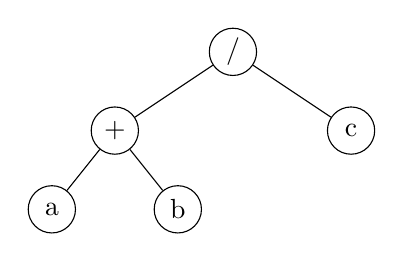
\begin{tikzpicture}[level distance=1cm, every node/.style={circle,draw,minimum size=6mm,inner sep=1pt},
 level 1/.style={sibling distance=3cm}, level 2/.style={sibling distance=1.6cm}]
\node {$/$}
 child { node {$+$} child { node {a} } child { node {b} } }
 child { node {c} };
\end{tikzpicture}
\end{column}
\begin{column}{0.5\linewidth}
\begin{itemize}
    \item Az operátorok a belső csúcsok, az operandusok a levelek.
    \item Postorder bejárása a lengyel formát adja: \texttt{a b + c /}
    \item Inorder bejárása a zárójelezés nélküli alakot adja.
\end{itemize}
\end{column}
\end{columns}
\end{frame}

\begin{frame}{Teljesen zárójelezett alak}
Minden zárójelpár pontosan egy operátort és annak bal és jobb operandusát tartalmazza.

\vspace{2mm}
\begin{tabular}{ll}
$a+b$ & $(a+b)$\\
$a+b*c$ & $(a+(b*c))$\\
$(a+b)/c$ & $((a+b)/c)$\\
$a\text{\textasciicircum}2/(x-y)$ & $((a\text{\textasciicircum}2)/(x-y))$\\
\end{tabular}

\vspace{2mm}
Fa építése: a legkülső zárójelpár operátora lesz a gyökér, a bal és jobb operandusból rekurzívan építjük a részfákat; a nem zárójelezett operandus levél.
\end{frame}

\begin{frame}[t]{Feladat: kifejezésfa építése}
Építsük fel a $((a+b)*c)-(d/(e+f))$ kifejezés fáját, majd a lengyel formából is:

\texttt{a b c * + d e / -}
\end{frame}

\begin{frame}[t]{Feladat: kiírás zárójelezve}
Adott egy láncoltan ábrázolt kifejezésfa. Készítsünk rekurzív algoritmust, mely kiírja a kifejezés teljesen zárójelezett alakját.
\end{frame}

\begin{frame}[t]{Szorgalmi házi feladat}
Adott egy láncoltan ábrázolt bináris fa. Készítsünk rekurzív algoritmust (nem szintfolytonos bejárással), mely megadja a legkisebb szintszámot, ahol a fának levele van. Üres fára $-1$-et adjon vissza.
\end{frame}

\end{document}
